%\documentclass{acm_proc_article-sp}
\documentclass[a4,twocolumn,10pt]{article}

\usepackage[utf8x]{inputenc}

\usepackage{graphicx} 
\usepackage{subfigure}
\usepackage{paralist}
\usepackage{hyperref}
\usepackage{amsfonts}
\usepackage{mathtools}
\usepackage{url}
\usepackage{xspace}
\usepackage{booktabs}

\usepackage{tikz}
\usetikzlibrary{decorations.pathreplacing}
\newcommand{\tikzmark}[1]{\tikz[overlay,remember picture] \node (#1) {};}

\usepackage[draft,nomargin,footnote]{fixme}

\graphicspath{{figs/}}

\newcommand{\eg}{{\textit{e.g.\xspace}}}
\newcommand{\etal}{{\textit{et al.\xspace}}}
\newcommand{\ie}{{\textit{i.e.\xspace}}}

\title{New Insights on the Role of Context in the Perception of a Human-like Robot}

\author{
Ashish Ranjan Jha, Kshitij Sharma, Séverin Lemaignan, Pierre Dillenbourg\\
CHILI Lab, École Polytechnique Fédérale de Lausanne\\
\url{firstname.lastname@epfl.ch}
}

\begin{document}
\maketitle
\begin{abstract}

What leads us to attribute human-like characteristics to robots? The physical
appearance of the robot, as well as the design of the behaviours, certainly play a key
role. This paper however evidences another mechanism at play, more subtle and partially
unconscious: the \emph{cognitive context}\fxwarning{cognitive context, really?}
of the interaction.

To study this effect, we propose an original methodology based on eye-tracking
and a serie of stimuli that are visually identical and yet elicit different
assumptions regarding the cognitive capabilities of the robot. We then correlate
the gaze patterns with established questionnaires that assess anthropomorphic
attributions.

\begin{inparaenum}[\itshape a\upshape)]
As a result, we show that \item gaze patterns correlate with post-hoc anthropomorphic
attributions, and hence, eye-tracking can be used as a novel \emph{in-the-moment}
metric of anthropomorphism, \item fixations on the robot's head are a good
predictor of anthropomorphic attributions, \item simple context priming is sufficient
to elicit significantly different anthropomorphic attributions.
\end{inparaenum}

This last item has noteworthy implications regarding the design of human-like human-robot
interactions, and we propose to discuss them at the end of the article.

%We present a study that investigates the relation between anthropomorphism and
%gaze patterns of the observers. Anthropomorphism usually refers to attributing
%human-like characteristics by a human to a non-human agent/entity; in this
%study, the non-human entity is a robot. 
%
%We hypothesize that while observing a human-robot interaction in a particular
%setting, the observer develops an anthropomorphic behavior for the robot.
%Moreover, the resulting anthropomorphism can be correlated with the gaze
%patterns of the observer as well as with the recorded response of the
%participants about their experience of the interaction (in the form of a
%questionnaire), both before and after the experiment. We try to seek the answer
%to the question whether anthropomorphism goes beyond the shape and body
%features, and we indeed observe that just by the use of audio commands of
%different cognitive levels, anthropomorphic attitude gets affected. We obtain
%two other useful results. First, eye tracking serves to be an effective way for
%measuring anthropomorphism. Second, in our study, the standard anthropomorphism
%tests are also validated such as, a person who can anthropomorphize more, in
%general, responds to a human scene and a robot scene in a similar manner.
%
%We observe a significant increase in the gaze fixations over the actor's head
%for a high cognitive scene compared to a low cognitive scene. We also achieve
%the result that the high cognitive interaction scenarios are capable of inducing
%anthropomorphic behavior more than the low cognitive scenarios.

\end{abstract}

%\keywords{anthropomorphism, eye tracking, gaze patterns, robot}

\section{Introduction}

It is widely accepted that anthropomorphism describes a set of human-like
features of a robot (like shape, speech capabilities, facial expression).
Lemaignan~\etal~\cite{lemaignan2014dynamics}  refer to these characteristics as the
anthropomorphic design of the robot .  Anthropomorphism, as described by
Lemaignan~\etal, refers to the social phenomenon that emerges from the
interaction between a robot and an user. According to Epley~\etal
\cite{epley_when_2008},
this includes for instance emotional states, motivations, intentions ascribed by
the user to the robot. 

Anthropomorphism is seen as a special kind of social (human-like) engagement
with robots. We made an attempt to analyze anthropomorphism in a
\textit{human-robot} interaction by utilizing the gaze patterns of the
participants (who watched this interaction). These gaze patterns were compared
to the gaze patterns for a similar \textit{human-human} interaction setting. The
``human'' part of the human-robot and human-human interactions mentioned above
is only in the form of an audio command and not physically present in the scene.
Hence, we represent the interactions with $\mathcal{R}$ and $\mathcal{H}$ in
this report for the human-robot and human-human settings respectively.

There were four hypotheses made in this experiment. We hypothesized
(\textbf{H1}) that the gaze patterns can distinguish between $\mathcal{H}$ and
$\mathcal{R}$ interaction scenarios. Further, this gaze pattern difference can
be denoted as the distribution of gaze on areas of interest in the scene.
Secondly, we hypothesized (\textbf{H2}) that the difference in gaze patterns
between $\mathcal{H}$ and $\mathcal{R}$ conditions
($\delta_{\mathcal{H},\mathcal{R}}$) correlate with the participants'
\textit{initial capital of anthropomorphism} (ICA), where the ICA was measured
as the sum of the ratings (responses) given by the participants to the questions
of the pre-questionnaire. This means that for participants whose ICA is low, the
gaze patterns should be significantly different for the $\mathcal{R}$ as
compared to that for the $\mathcal{H}$ videos and vice-versa.

We also hypothesized (\textbf{H3}) that the gaze patterns can distinguish
between high-cognitive and low-cognitive tasks. Finally, we hypothesized
(\textbf{H4}) that the cognitive priming will have an effect on the difference
between ICA and \textit{adaptive anthropomorphic perception} (AAP) \ie
$\Delta_{ICA,AAP}$ (where AAP is measured for the post-questionnaire in a
similar way as the ICA).

We used stationary eye tracking technique for tracking the gaze patterns and
``Nao", a robot manufactured by Aldebaran Robotics was used in this
experiment. We prepared the scripts for the robot using Choreographe. The
interactions were recorded as videos and were then shown to the participants.
The scenarios that were covered in the videos were aimed at eliciting the
human-like or high-cognitive (HC) feelings for the robot in one setting and
robot-like or low-cognitive (LC) feelings in the other setting. For example, we
had a scene, where the robot is asked by the human to \textit{``pick up the
brown toy"} and in another scene, with the same video, the robot is asked to
\textit{``pick up its favorite toy"}. We tried to keep our distribution of
participants uniform across all variations of the scenarios to avoid any biases
to our results. The change in the feelings of participants were recorded in the
form of response to two questionnaires before and after the experiment. The
difference in the response of the two questionnaires was used to measure the
impact the videos had on the participants. 

As mentioned earlier, the human element in the $\mathcal{R}$ interaction was in
the form of only a human voice, basically a command given by the human to the
robot. This command (\eg ``pick up the brown toy") was used to prime
the context thereby classifying the scenario as LC or HC. Initially we had three
different scenarios where the robot/human was asked:

\begin{enumerate}
    \item to pick up a toy
    \item to point to a sound/noise
    \item to show some movements (or dance)
\end{enumerate}

Differing from first two scenarios, the third scenario had only one object in
the video \ie~the actor (human or robot). In the first two scenarios, a
participant could make gaze transitions, say, between the robot and the toys for
the first scene. In contrast, in the third scene, a participant could only look
at the robot showing its movements. The third scene, hence, was more related to
observing the various body movements and was not helpful in identifying
differences in gaze patterns based on LC and HC scenarios and therefore, we did
not consider it for our study. First, a pilot experiment was conducted with a
small number of participants and then a full-fledged experiment was carried out.

\section{Related Work}

In a human-robot interaction, studying anthropomorphism would essentially mean
the assessment of human's tendency to engage in a human like way with robots
(that are not deliberately made to buttress such relationship). In broader
terms, anthropomorphism can be understood as the phenomenon between a human and
a non-human, where the human tends to attribute human characteristics to the
non-human in order to establish a meaningful contact\cite{fink2014dynamics}. But
there have been a plethora of definitions of anthropomorphism not only across
but within disciplines\cite{duffy_anthropomorphism_2002}. Even
within HRI (human robot interaction) and robotics, there has not been a single
unique definition of anthropomorphism, but a variety of them.
Bartneck~\etal\cite{bartneck_measurement_2008} refer to it as \emph{``the
attribution of a human form, human characteristics, or human behavior to
nonhuman things such as robots, computers, and animals."} Contrarily,
Waytz~\etal\cite{Waytz2010} apply a more psychological-cognitive view and
define anthropomorphism as \textit{``a process of inductive inference whereby
    people imbue the real or imagined behavior of other agents with human like
    characteristics, motivations, intentions, or underlying mental states".} 

Etymologically, anthropomorphism is a term composed of two Greek words :
\textit{anthropos} for ``man" (or ``human") and \textit{morphe} for ``from /
structure" (or ``shape"). Although anthropomorphism" literally would mean
``human form", it should \textit{not} be used to refer to the \textit{form/
design} of a non-human agent. The term \textbf{anthropomorphic design} would
rather be a better choice to refer to imitating human-like form / design of a
robot. Bartneck and Forlizzi\cite{bartneck_shaping_2004} recommend that \emph{form}
refers not just to the physical shape of a robot but to all ascertainable parts
of it. Therefore, ``form" could be seen as the overall expression of the robot,
that includes its shape, materials, and behavioral characteristics.
Anthropomorphic form can be broadly classified, but there is no fine line
dividing these categories: anthropomorphic, caricatured, functional,
zoomorphic (Fong \etal \cite{fong_survey_2003}).

Another key aspect in the discussion of anthropomorphism is the change in
people's perception of robots over their time of interaction with robots. And as
the perception changes, the tendency to anthropomorphize the robot is likely to
change. Such a gap related to the perceived agency of the robot was discussed by
Takayama \cite{takayama_perspectives_2012}. She noticed that among people who
own a robot, while some people perceive their robot as an agentic object, others
feel  it as only a plain machine. In order to distinguish between these two
patterns and make sense out of them in relation to people's perception of robots
in general, Takayama differentiated between what she calls an
\emph{in-the-moment} and a \emph{reflective} perspective on agency. Hence, an
\emph{in-the-moment} perspective would refer to one's most immediate
response/sense in a given situation. On the other hand, a \emph{reflective}
perspective would indicate one's reaction/sense of a situation based on a more
in-depth  consideration and contemplation \cite{takayama_perspectives_2012}. 

Quite often, these two distinctions are not considered differently, leading to
errors and confusions.  In other words, in an initial phase of interaction with
a non-human agent, people might respond ``mindlessly" instead of responding
consciously\cite{nass_machines_2000}. Only post a due amount of
time of, what is generally called as ``familiarization" with the robot, one
might respond in a more reflective manner instead of an in-the-moment reaction.
This can be demonstrated by the fact that when participants who had interacted
with a technology, were asked about whether the interaction with the technology
was in a human-like way, most of them denied this which shows the reflective
perspective . However, the same participants had actually reacted ( in the
moment of the interaction) to the system in many ways that were quite close to
how they would react to people\cite{reeves_media_1996}.

\subsection{Novel Contributions}

The study and results presented in this article lead to two main contributions:
new insights on the impact of the cognitive context of the interaction on the
perception of a robot by humans; a novel unbiased\fxwarning{correct?}
methodology based on eye-tracking to measure anthropomorphic attributions during
a running human-robot interaction.

Our first contribution extends our understanding of the attribution of
human-like characteristics to robot by exploring the role of the interaction
context. As we will show in the article, it appears that \textbf{even relatively
subtle context priming may lead to significantly different anthropomorphic
perceptions of the exact same robot, performing the exact same task}, as
confirmed both by distinct gaze patterns, and different reported perceptions in
questionnaires. As far as we know, this effect had not been previously
evidenced.

This leads to a second-order effect that we also evidence here: depending on the
cognitive context, the tendency to attribute human-like characteristics to robot
\textbf{evolves} in significantly different ways: after observing a robot in a
context that pre-suppose deeper cognitive capabilities, \textbf{people increase
their general tendency to anthropomorphize robots} compared to a shallow
cognitive context, even though the robot appearance and behaviour is the exact
same.

The second contribution is a methodological one: we present in this article
\textbf{a novel technique to assess anthropomorphic projections that relies on a
biometric measurement (eye-tracking) to compare gaze fixation durations on
the face of the robot}. We cross-validate this new metric with existing,
established, questionnaires. Compared to current techniques (post-hoc
annotations of videos and questionnaires), this new approach is objective,
is less impacted by experimental biases (like the \emph{observer effect},
where the subject's behaviour is impacted by the fact he/she knows that
he/she is observed) and take place during the interaction itself
(\emph{in-the-moment} measurement).

Besides, we also introduce a new kind of visual stimuli, specifically designed
to study the impact of non-appearance, non-behavioural related effects on the
human-like perception of robots. We make these video stimuli available to the
community, and therefore invite our colleagues to reproduce our experimental
results.


As a whole, we believe that this article provide a solid contribution, both in
terms of methodology and experimental evidence, to our understanding of one of
the intricate psychological effects that come to play when humans and robots
interact.

\section{Experimental Design}

This study is build as an eye-tracking experiment (mainly measuring fixation times on
various body parts) where participants watch short videos of an agent (either a
robot or a human) performing a very simple task (like picking an object), in
two different \emph{socio-cognitive contexts}. These contexts, created by priming
and/or audio cues, are designed to elicit either a shallow cognitive context
(that participant would refer as a \emph{machine-like} situation) or a deeper
cognitive context (refered as a \emph{human-like} situation).

\subsection{Conditions}

The study follows a 2x2 design, summarized in table~\ref{table:design}. Our two
independent variables are the level of socio-cognitive context (\emph{shallow
cognitive context} vs \emph{deep cognitive context}) and the nature of the
agent appearing in the stimulus (a \emph{robot}, eliciting a \emph{human-robot} interaction
situation, or a \emph{human}, eliciting a \emph{human-human} interaction
situation).

\begin{table}
    \centering
    \small

    \tikzmark{top}

    \tikzmark{left}
    \begin{tabular}{l|p{2.5cm}|p{2.5cm}}
        & \tikzmark{top1} Shallow cognitive context & Deep cognitive \tikzmark{top2} context  \\
        \hline
        \tikzmark{left1} Robot & {\bf A}: \emph{``Pick the brown toy''} & {\bf A}: \emph{``Pick your favorite toy''} \\
                               & {\bf B}: \emph{``Point at the noise''} & {\bf B}: \emph{``Point at the crying baby''} \\
        \hline
        \tikzmark{left2} Human & {\bf A}: \emph{``Pick the brown toy''} & {\bf A}: \emph{``Pick your favorite toy''} \\ 
                               & {\bf B}: \emph{``Point at the noise''} & {\bf B}: \emph{``Point at the crying baby''}\tikzmark{bottom} \\
        \end{tabular}

    % draw the over- and side-braces
    \begin{tikzpicture}[overlay, remember picture]

        \draw [decoration={brace,amplitude=0.5em},decorate,thick]
            (top -| top1.west) --  (top -| top2.east) node[midway, above=0.5em] {\scriptsize between subjects};

        \draw [decoration={brace,amplitude=0.5em},decorate,thick]
            (left |- bottom) --  (left |- left1.north) node[midway,above=3em,left=1em,rotate=90] {\scriptsize within subject};
    \end{tikzpicture}
    %%%

    \caption{\small The study follows a 2x2 design: the \emph{robot} vs
        \emph{human} condition is within subject, while the \emph{shallow
        cognitive context} vs \emph{deep cognitive context} is between subject.
        Two stimuli (\emph{``toys''} scene, {\bf A}, and \emph{``noise''} scene,
        {\bf B}) were shown to the participants, introduced by brief verbal
        commands, reproduced in the table. While visually identical (see
        screenshots on figure~\ref{fig:stimuli}), the stimuli were introduced
        with different commands in the two conditions \emph{shallow} and
        \emph{deep cognitive
        context}.}

    \label{table:design}
\end{table}


\subsubsection{Dependent Variables}

We have a dependent variable that is the difference between the ICA and AAP.
This represents how much a participant has been affected by watching the videos
because it reflects the difference in the response of a participant in the pre
and post questionnaires.


\subsection{Video Stimuli}

Four different video stimuli where filmed (figure~\ref{fig:stimuli}): two
different tasks (picking a stuffed animal, refered hereafter as the
\emph{Picking} task, and pointing towards a source of sound, refered as the
\emph{Sound} task) acted either by a human or a robot. Video stimuli were
realised in studio conditions. All videos followed the same simple structure: an
initial audio command (spoken by an invisible person), followed by the task
being executed.

The human actor was instructed to follow as closely as possible the actions and
attitudes of the robot (left/right glances, hesitations\ldots), while keeping a
natural, \emph{human-like} general behaviour.  Hence, the length of human videos
(57 seconds in total for the two tasks) was shorter than robot videos (110
seconds) due to the robot being usually slower in performing actions (in
particular walks) compared to human.

The audio (and audio only) of these four videos was edited to create two sets of
stimuli: one for the \emph{shallow cognitive context} condition, one for the
\emph{deep cognitive context} condition. The audio editing consisted in
inserting \emph{different commands} to initiate the tasks (reported in
table~\ref{table:design}), and, in the \emph{Sound} task, to use as sound source
either a repetitive bip (\emph{shallow cognitive context}) or the sound of a
crying baby (\emph{deep cognitive context}).

\begin{figure}
    \centering
    \subfigure[\emph{Picking} task, robot condition]{
        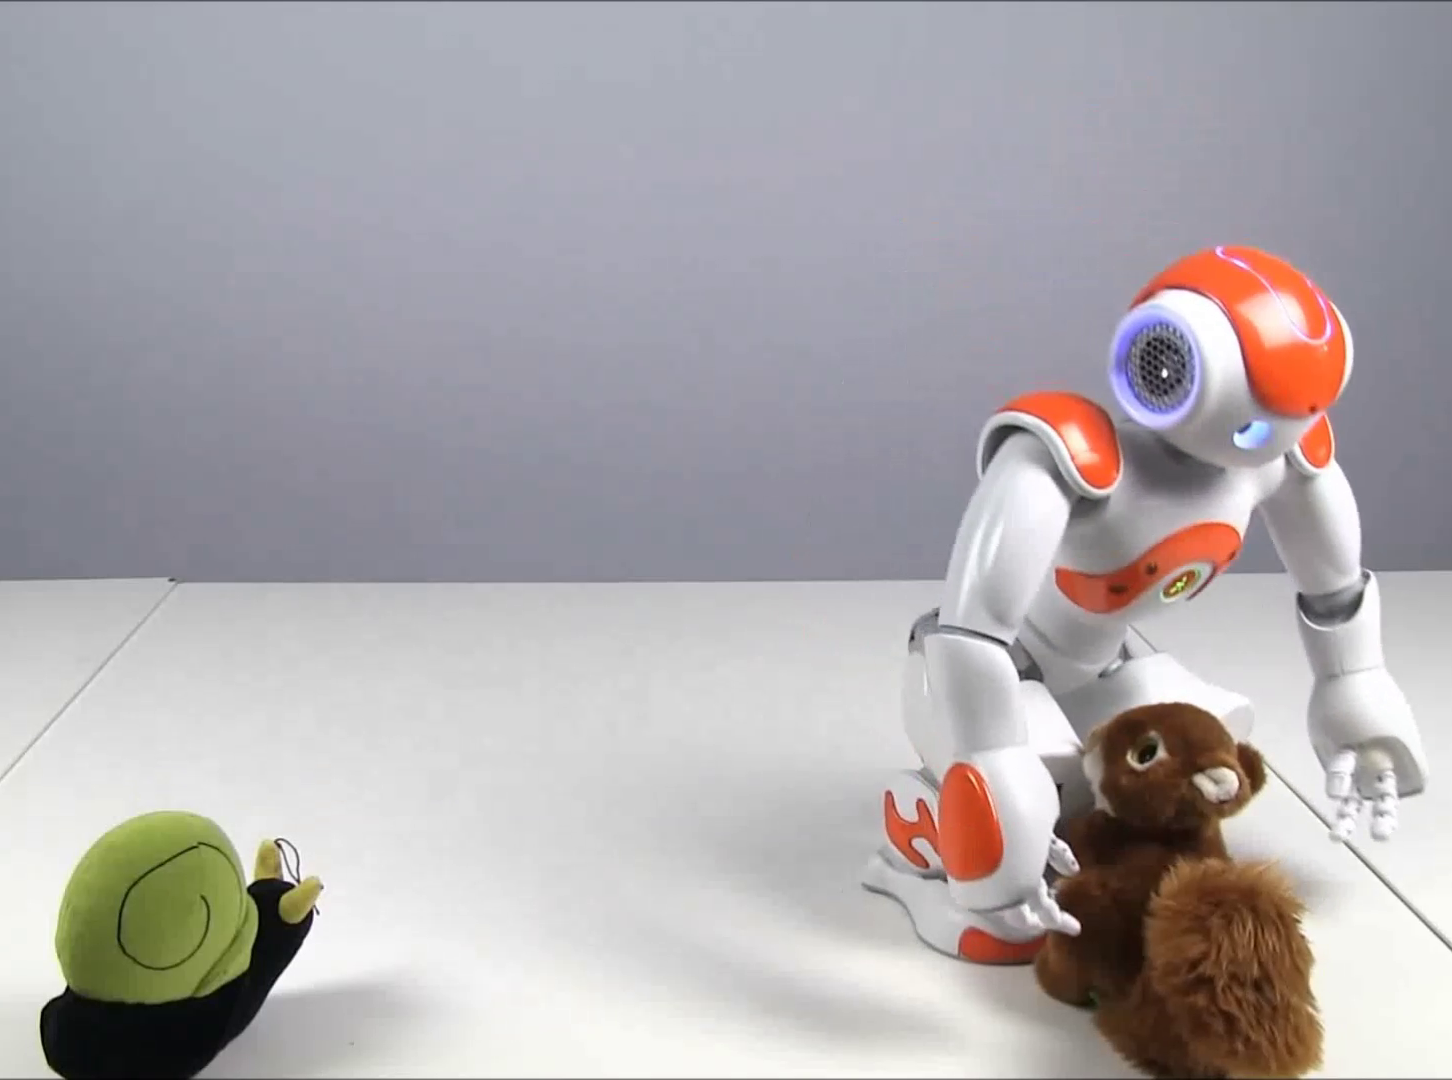
\includegraphics[height=3cm]{stimulus-robot-toys}
    }
    \subfigure[\emph{Picking} task, human condition]{
        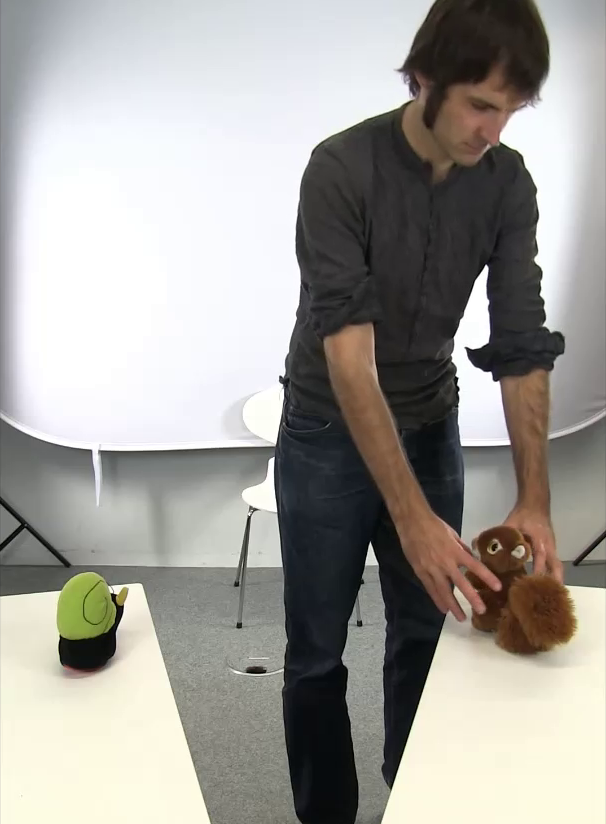
\includegraphics[height=3cm]{stimulus-human-toys}
    }

    \subfigure[\emph{Sound} task, robot condition]{
        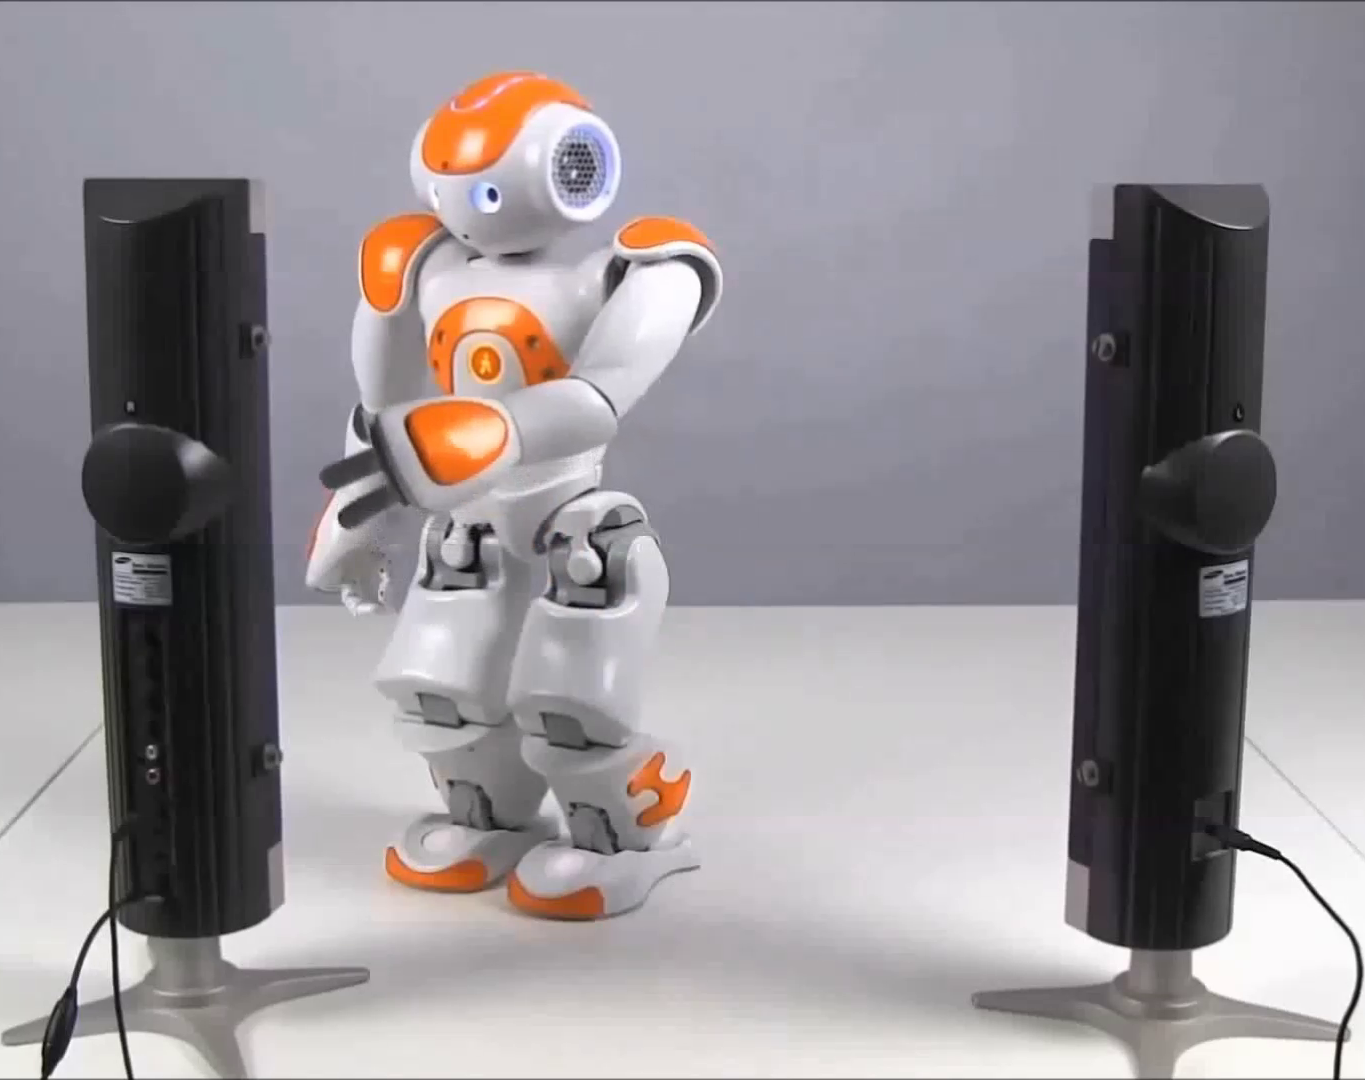
\includegraphics[height=3cm]{stimulus-robot-noise}
    }
    \subfigure[\emph{Sound} task, human condition]{
        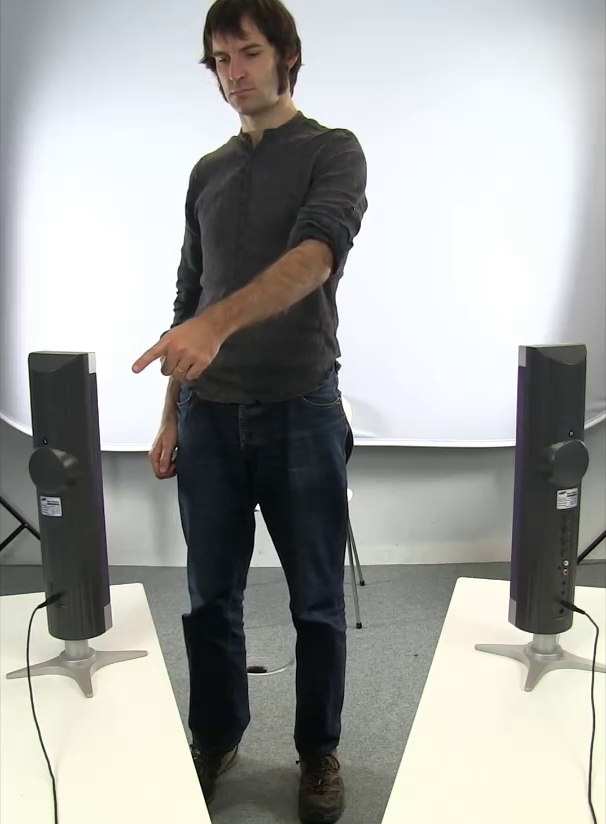
\includegraphics[height=3cm]{stimulus-human-noise}
    }


    \caption{\small Screenshots of the 2x2 stimuli. Note that the images above have been
    slightly cropped: the original video are framed so that the agent (robot or
    human) always remains entirely visible.}
    \label{fig:stimuli}
\end{figure}




\section{Course of the study}

We did a pilot test using 10 participants first, and then after some
modifications, we did the final experiment on 40 participants.

\subsubsection{Participants}

Participants on an average were around 21 years of age (SD=4.5). Among 40
participants, 21 were females and 19 were males.

The participants were recruited amongst students of our university. To avoid students
with a higher familiarity with robots and artificial intelligent systems,
Computer Science and Electronics curriculum were excluded. This was \textit{a
posteriori} comforted as per the questionnaire responses: no
participants\fxwarning{to be checked}
reported itself as being familiar with robots and only a few\fxwarning{how
many?} out of 40 had ever owned a robot.

It took
approximately 15 minutes per participant for one experiment session.  Each
participant was invited for only one session. 

The \emph{shallow} vs \emph{deep cognitive context} condition was between
subject: Out of the 40 participants, 22 watched the \emph{deep cognitive}
tasks and 18 watched the \emph{shallow cognitive} tasks.

The \emph{robot} vs \emph{human} condition was within subject. The order of
stimuli presentation was counter-balanced over the 40 participants.

\subsubsection{Consent Form}

Before the experiment, participants were made to read, understand and sign a
standard consent form.

\subsubsection{Initial Interaction}

After the pre questionnaire, we kept a 2 to 3 minutes session for initial
interaction, where we let the participant spend some time with Nao.
The purpose of this interaction was to familiarize the participants with the
robot and mitigate the novelty effect, so that they do not get surprised seeing
a robot for the first time in the videos.

\subsubsection{Pre-questionnaire}

Participants were asked to fill the 49 questions questionnaire right after the
initial interaction.

\subsubsection{Videos}

After filling the pre-questionnaire, participants watched the $\mathcal{R}$ and
$\mathcal{H}$ interaction videos.

\subsubsection{Post-questionnaire}

After watching the videos, participants were asked to fill the post
questionnaire, which was the last step in the procedure of this study.

\subsubsection{Reward}

Each of the participants were given a reward equivalent to CHF 10.

\begin{figure}
    {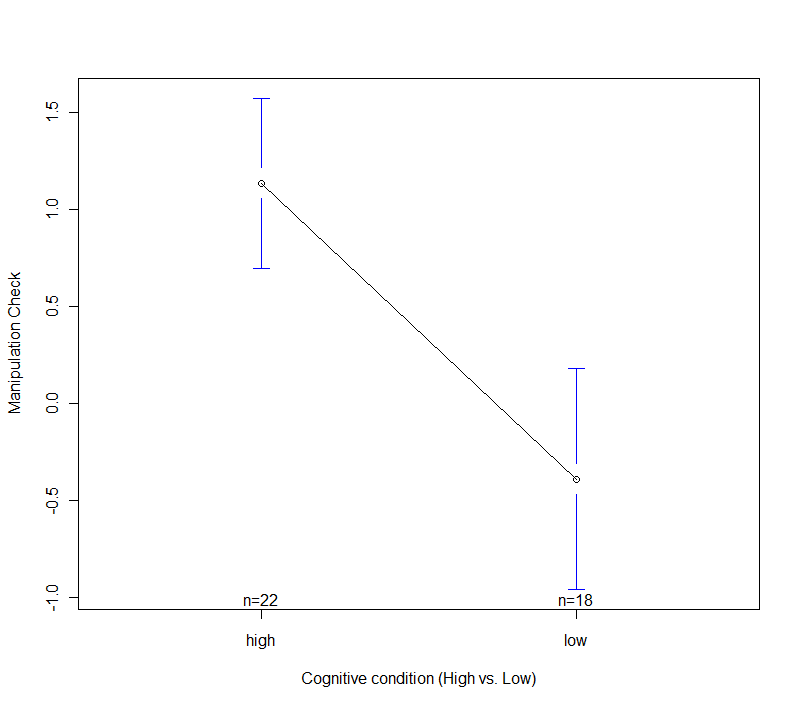
\includegraphics[width=3.3in]{ManipulationCheck}}
    \caption{Manipulation check}
    \label{fig:ManipulationCheck}
\end{figure}


\subsection{Data Collection}

\subsubsection{Gaze variables}

\paragraph{Areas Of Interest(AOI)}

Among the two scenarios, the first was one was about the robot/human picking up
a toy and the second one about pointing to the noise. As seen in
figure~\ref{fig:aoi-toys}, in
the first scenario, we had 10 AOIs: 1 for the actor's (robot/human) head, 2 for
arms (left and right), 2 for hands, 2 for legs and 1 for torso, and also 2 for
the two toys (green and brown). Similarly, as shown in
figure~\ref{fig:aoi-noise}, we had 10
AOIs for the second scenario, where the 2 AOIs for toys were replaced by two
speakers that produced sound. We fetched the gaze patterns that fall into one of
these 10 AOIs and analyzed the gaze distribution among them.

\begin{figure}
    \centering
    \subfigure[\emph{Picking} task, robot condition]
    {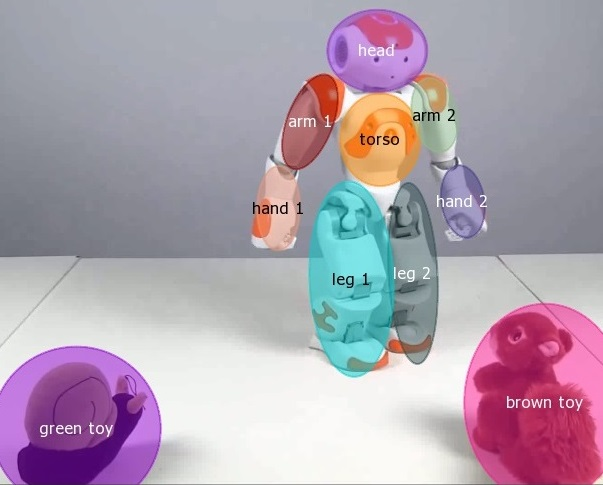
\includegraphics[width=0.8\columnwidth]{aoi-robot}\label{fig:aoi-toys}}

    \subfigure[\emph{Sound} task, human condition]
    {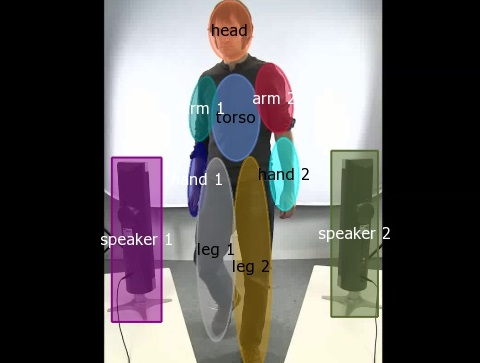
\includegraphics[width=0.8\columnwidth]{aoi-human}\label{fig:aoi-noise}}

    \caption{Areas of interest used for the gaze analysis}
    \label{fig:aoi}
\end{figure}

\paragraph{Proportion of time on the AOIs}

We fetch only the gaze patterns that fall into one of these 10 AOIs and analyze
the gaze distribution among them based on the proportion of time spent in
viewing each of these AOIs. This helps in drawing comparisons between various
objects present in the scene. 

\paragraph{Difference in gaze patterns}

An important data to be obtained here is $\delta_{H,R}$. This is calculated by
taking the difference between the ratio of net dwell time of an AOI and the AOI
fixation coverage summed over all the AOIs in the scene. Hence,
$\delta_{\mathcal{H},\mathcal{R}}$ is expressed as a ratio in the range of 0 to
1. Similarly, the differences between gaze patterns of two participants, where
one watches the LC task, given by $\delta_{low}^{\mathcal{H},\mathcal{R}}$ and
the other watches the HC task, given by
$\delta_{high}^{\mathcal{H},\mathcal{R}}$ are important gaze variables.


\subsubsection{Questionnaires}

\paragraph{Pre-questionnaire}

The participants were asked to fill a questionnaire which had 49 questions. The
responses to the questions were scaled in the 5-point likert scale, numerically
ranging from -2 to 2. The questionnaire had ten questions from the 10 item
big-five personality questionnaire. And then there were questions taken from
godspeed questionnaire and other questionnaires. Please refer to the appendix
for a sample questionnaire used in this study. The ICA was calculated as the sum
of the ratings/points provided by the participants for questions 30 to 39 as
these were the questions most closely resembling anthropomorphism. In this
report, we refer to this questionnaire as the pre-questionnaire \ie before the
experiment, and it typically took 5 minutes for participants to fill it. 

\paragraph{Post-questionnaire}

There was another questionnaire form that was almost identical to the
pre-questionnaire that the participants had to fill after watching the videos.
This questionnaire typically took 3 to 4 minutes to fill and we refer to this as
the post-questionnaire. A sample is provided in the appendix of this report.
Based on the responses filled in this questionnaire, the AAP was calculated as
the sum of the ratings/points provided by the participants for questions 17 to
26 (similar to ICA).


\subsection{Course of the study}

\section{Results}

Based on the experiments conducted on 40 participants in the $\mathcal{H}$ and
$\mathcal{R}$ interactions across LC and HC conditions, we have the following
results. (The detailed statistics and code used for obtaining the results are
available here : \url{https://github.com/chili-epfl/anthropomorphism-eyetracking})

\subsection{General Biases}

While testing for all the 4 hypotheses, we observed no significant bias with
respect to age, gender, EPFL status, familiarity with robot and robot ownership
of the participants, \ie there was no correlation found between these factors
and the gaze patterns in the videos.

\subsection{Manipulation check}

In our post-questionnaire, we had a question asking the participants about
whether the video has a robot kind of task or a human kind of task on a scale of
-2 to 2 where -2 refers to robot kind of task. As can be seen in figure 2, we
got a significant correlation in this manipulation check (F[1,36] = 20.42, p <
.01) which means that the participants that were shown the LC videos identified
the task as the robot-like and participants watching HC videos perceived the
tasks as more human-like. 




\subsection{H1: Gaze patterns for Human vs Robot}

Among the 10 AOIs, we grouped the AOIs corresponding to the actor into 4
categories : Head, Arm (containing both arms and hands), Torso, Leg(containing
both legs). And this is the result that we obtained from the ANOVA between gaze
patterns on the AOIs versus the $\mathcal{H}$ and $\mathcal{R}$ conditions :

\textit{\textbf{head}}: the fixations on the head for the $\mathcal{H}$ scene
were observed to more than that for the $\mathcal{R}$ scene (F[1,36] = \ 6.60, p
< .05)

\textit{\textbf{arm}}\ : the fixations on the arms for the $\mathcal{H}$ scene
were also greater than that for the $\mathcal{R}$ scene (F[1,36] = 18.65, p <
.01)

\textit{\textbf{leg}}\hspace{0.18cm} : the fixations on the legs were much lower
for the $\mathcal{H}$ scene as compared to the $\mathcal{R}$ scene (F[1,36] = \
2.89, p < .1)

\textit{\textbf{torso}} : the fixations on the torso was more for the
$\mathcal{H}$ scene than for the $\mathcal{R}$ scene (F[1,36] = \ 3.54, p < .1) 

\subsection{H2: Difference in gaze patterns vs ICA}

We got a significant correlation between $\delta_{\mathcal{H},\mathcal{R}}$ and
the ICA. As can be seen in figure 3(a), there is a significant negative
correlation between the two quantities (Pearson Correlation Coefficient = -0.42,
p < .01).

\begin{figure}
    \subfigure[Difference in gaze patterns vs ICA]
    {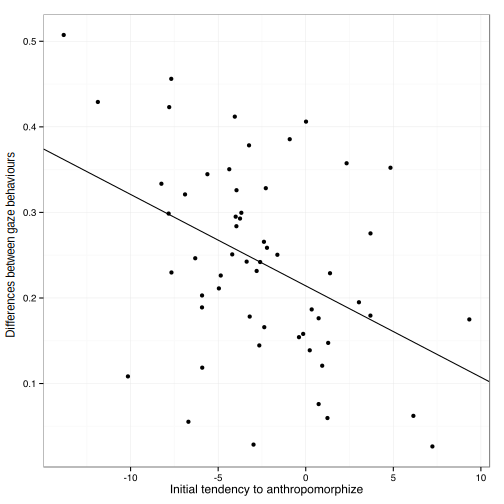
\includegraphics[width=3.3in]{H2}\label{GazeDifference-vs-ICA}}
    \subfigure[Gaze patterns for high vs low condition]
    {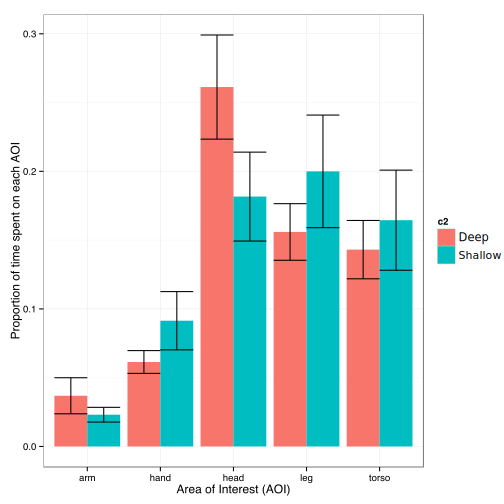
\includegraphics[width=3.3in]{GazeHighLow}\label{GazeHighLow}}
    \subfigure[Difference between ICA and AAP versus High/Low]
    {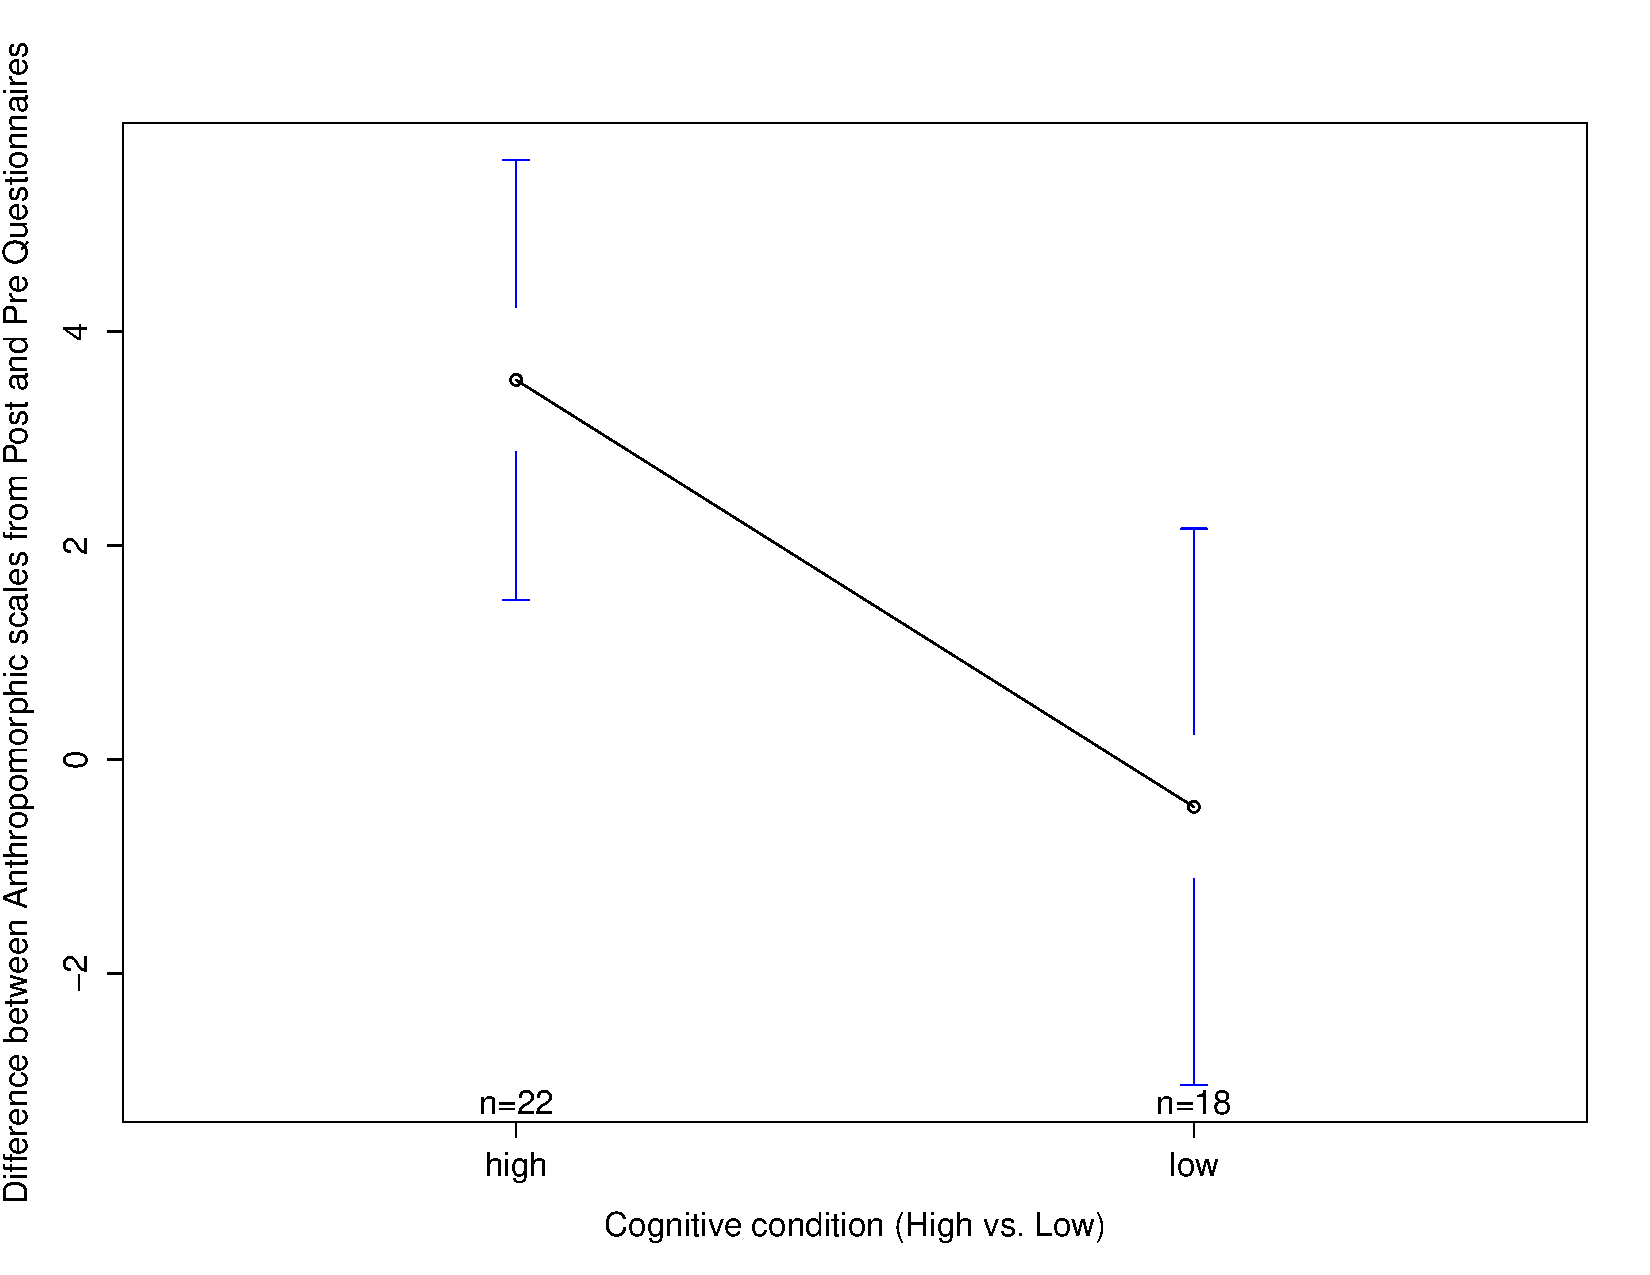
\includegraphics[width=3.3in]{H4}\label{ICAtoAAPImprovement}}
    \caption{Hypotheses H2, H3, H4}
\end{figure}

\subsection{H3: Gaze patterns for high vs low cognitive condition}

This test was done only for $\mathcal{R}$ scenario as the $\mathcal{H}$ case is
by default a source of HC condition, hence, would not make a big impact in
changing the patterns across the LC and HC conditions. Based on ANOVA results,
taking just the 5 AOI groups (head, arms, hands, torso, legs) for the robot in
both LC and HC conditions, the fixations on the head in the HC condition was
found to be significantly higher than that in the LC condition (F[1,36] = 4.55,
p < .05). For all other AOI groups, the fixations across LC and HC were almost
the same. Figure 3(b) shows the distribution of proportion of time spent gazing
on the 5 AOIs for LC and HC conditions.

\subsection{H4: Difference between ICA and AAP versus High/Low}

ANOVA between $\Delta_{ICA,AAP}$ and the category of cognitive task
\ie HC or LC tells us that $\Delta_{ICA,AAP}$ is greater for HC tasks
than that for the LC tasks (F[1,36] = 6.54, p < .05). The results are shown in
figure 3(c).


\section{Discussion}

Based on the results that we obtained, we can now verify our four hypotheses.
For the first hypothesis where we state that the gaze patterns can distinguish
between $\mathcal{H}$ and $\mathcal{R}$ interaction scenarios, we get greater
amount of fixation on the head, arms and torso for the $\mathcal{H}$ scenario as
compared to the $\mathcal{R}$ scenario. This can be explained by the fact that
human is by default perceived as a high cognitive agent compared to a robot.
Hence, the proportion of time spent on looking at the head is more in case of
human videos as compared to robot videos. But the trend is opposite for legs.
This might be explained by the fact that the participants are fascinated by the
joints on the robot's legs \ie the novelty effect. Overall, this
result weakly validates our hypothesis.

In the second hypothesis, where we claim that $\delta_{\mathcal{H},\mathcal{R}}$
should correlate with the participants' ICA, we obtain in our results, a
significant negative correlation between the two quantities. From the negative
correlation, we can understand that if ICA is high, it means that the
\textit{human likeliness ascription} (HLA) is high (which means that there is a
greater tendency to anthropomorphize) which indicates that
$\delta_{\mathcal{H},\mathcal{R}}$ should be low. This supports our hypothesis
and can be explained by the fact that if HLA is high for a participant, then
even the $\mathcal{R}$ videos are quite human-like for such participant. 

The third hypothesis where we state that the gaze patterns can distinguish
between HC and LC tasks, can also be supported by our results. As can be seen in
figure 3(b), the proportion of time spent by participants on looking at the head
is significantly higher in HC task as compared to LC task. When participants
ascribe more anthropomorphic features to robot, they look more at the head than
when they ascribe less anthropomorphic features.

Finally for the fourth hypothesis where we state that the cognitive priming will
have an effect on $\Delta_{ICA,AAP}$, as seen in the results, $\Delta_{ICA,AAP}$
for participants that watched the HC task is greater than that for the
participants who watched LC task. This proves the fact that HLA was induced by
the videos and in fact, the HC tasks impose a greater HLA on the minds of
participants than the LC tasks. This shows the typical priming effect of the
audio command given in the beginning of the video and highlights the variation
in HLA based on the interaction scenario (LC versus HC) thereby supporting our
hypothesis. 

We analyze the gaze distribution in this study only based on the AOI net dwell
times . Apart from this, the gaze transition among AOIs can be another way of
fetching gaze patterns which is not used in this study.

\section{Conclusion}

In our experiment, we created two kinds of scenarios each for $\mathcal{H}$ and
$\mathcal{R}$ interaction and just by changing the audio commands (priming
effect), we replicated these videos to create a HC and a LC scene. We recorded
the gaze patterns of the 40 participants who were made to watch these videos and
also the participants were asked to fill two questionnaires before and after the
experiment. These data were analyzed and compared to our four hypotheses. We
hypothesized that one who anthropomorphizes more would have a similar reaction
to $\mathcal{H}$ and $\mathcal{R}$ conditions, and also that in the HC case, a
participant's fixations would be more on the head of the actor as compared to
that in the LC case. We also hypothesized that the HC scene would induce more
anthropomorphic attitude than the LC scene. We found that the results were
successful and supported our hypotheses. We also had another scenario where the
robot/human was asked to move/dance, but this scenario had only one object
(\ie the actor) showing movements, and hence participants would focus
more on seeing the movements leaving behind the cognition aspect, which made it
difficult to differentiate between the LC and HC cases and, therefore, we
discarded this scenario from our analysis.


\bibliographystyle{abbrv}
\bibliography{biblio}

%\appendix
%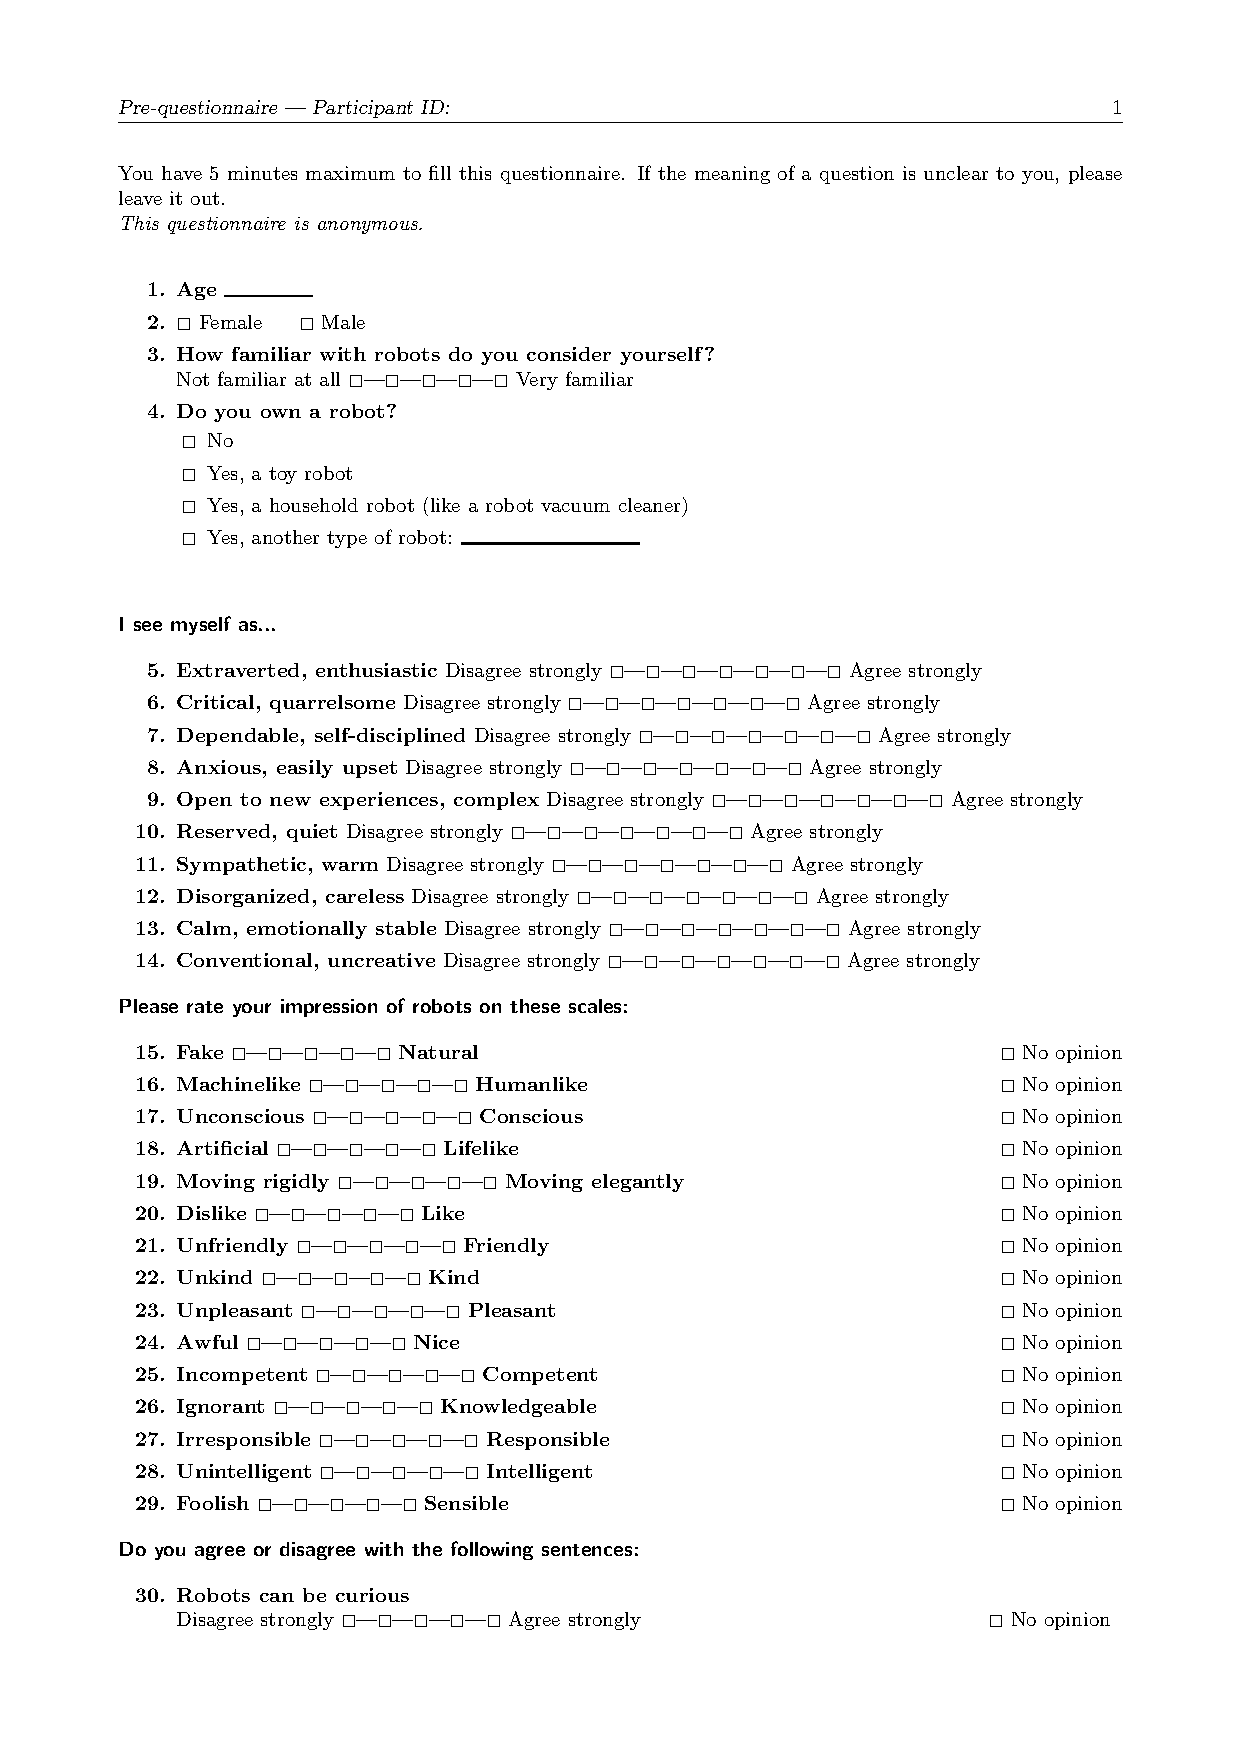
\includepdf[pages={1,2}]{pre-questionnaire.pdf}
%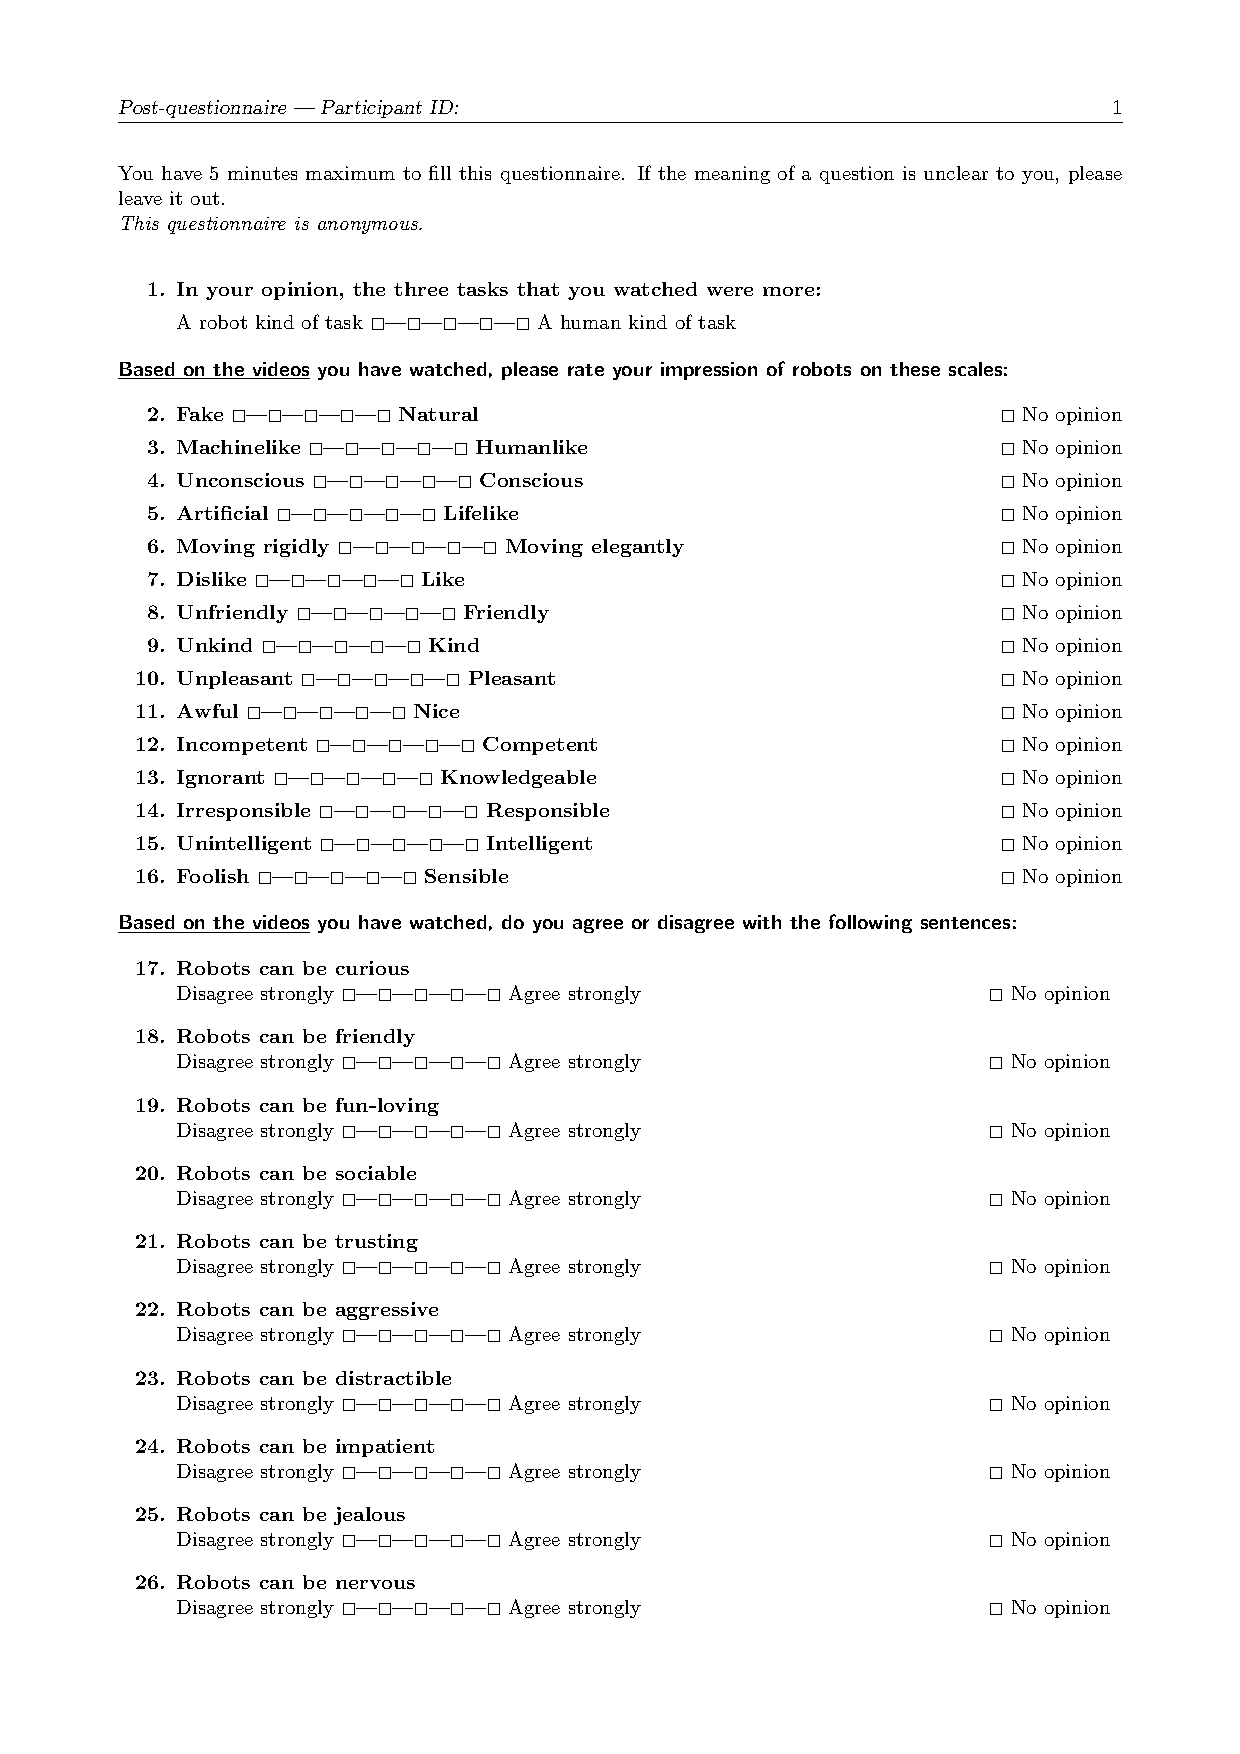
\includepdf[pages={1,2}]{post-questionnaire.pdf}

\end{document}
